\documentclass[tikz]{standalone}
\usepackage{booktabs}
\usepackage{tikz}

\usetikzlibrary{arrows,positioning,fit,shapes}


\begin{document}



\begin{figure}[!h]

\centering
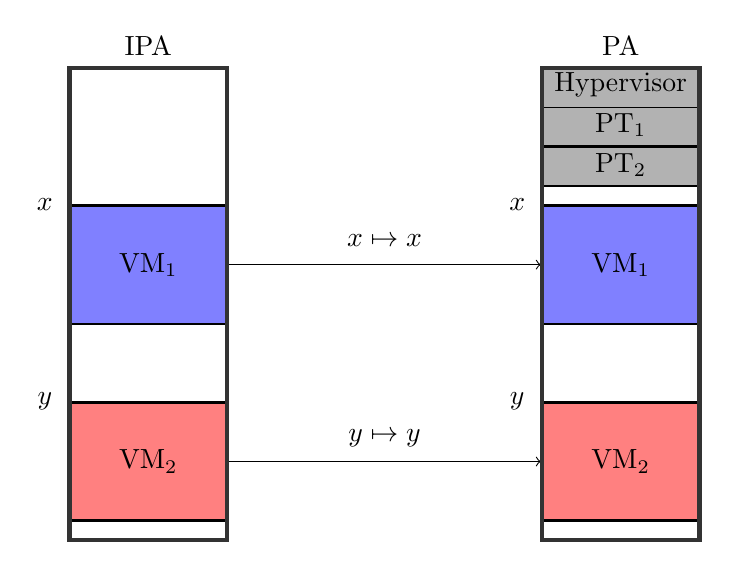
\begin{tikzpicture}[node distance=1cm, on grid]
 \tikzset{
pagetable/.style = {draw, minimum width=2cm,text height = 0.20cm},
memory/.style= {rectangle , draw = black, thick, minimum width = 2cm},
address space/.style = { rectangle, draw=black!80, ultra thick,minimum width=2cm,minimum height=6cm}}

\pgfdeclarelayer{foreground}
\pgfsetlayers{main,foreground}

    \begin{pgfonlayer}{foreground}
      \node [address space] (IPA)  at (-3,0) {};
      \node [address space] (PA) at (3,0) {};
      \node [above] at (PA.north) {PA};
      \node [above] at (IPA.north) {IPA};
    \end{pgfonlayer}
    \node [memory] (IP1)[fill = blue!50,minimum height = 1.5cm] at (-3,0.5) {VM$_{1}$};
    \node (X)[xshift = -3mm] at (IP1.north west) {$x$};
    \node [memory] (IP2)[fill = red!50,minimum height = 1.5cm] at (-3,-2) {VM$_{2}$};
    \node (Y)[xshift = -3mm] at (IP2.north west) {$y$};
    \node [memory] (PH)[fill = black!30,minimum height = 1.5cm] at (3,2.25) {};

    \node [pagetable] (PT1) at (3,2.25){PT$_{1}$};
    \node [pagetable] (PT2) at (3,1.75){PT$_{2}$};
    \node [above] at (PT1.north) {Hypervisor};

    \node [memory] (P1)[fill = blue!50,minimum height = 1.5cm] at (3,0.5) {VM$_{1}$}edge[<-] (IP1.east |- P1.west);
    \node (X')[xshift = -3mm] at (P1.north west) {$x$};
    \node [memory] (P2)[fill = red!50,minimum height = 1.5cm] at (3,-2) {VM$_{2}$}edge[<-] (IP2.east |- P2.west);
    \node (Y')[xshift = -3mm] at (P2.north west) {$y$};
    \node (E1)[minimum height = 0.5cm] at (0,0.8) {$x \mapsto x$};%edge[<-] (PT1.west);
    \node (E2)[minimum height = 0.5cm] at (0,-1.7) {$y \mapsto y$};%edge[<-] (PT2.west);

  \end{tikzpicture}
 \caption{Two-Stage Memory Translation}
  \end{figure}


\end{document}
